\documentclass[a4paper, 11pt]{article}
\usepackage{titlesec}
\usepackage{longtable}
\usepackage{listings}
\usepackage{graphicx}
\usepackage[fleqn]{mathtools}
%\titleformat{\subsection}[runin]{\bfseries}{\thesection}{1em}{}[]
%\titleformat{command}[shape]{format}{label}{sep}{before}[after]
\setlength{\mathindent}{0pt}
\lstset{language=C++}
\lstset{numbers=left, frame=shadowbox}
\lstset{breaklines}
\lstset{extendedchars=false}

\title{Experiment Report \\ \begin{large}--- Producer-Consumer Problem\end{large}}
\author{Name:Wang Xingyi StudentID:5140309531}
\date{\today}

\begin{document}
\maketitle
\section{Introduction}
In this project, we will design a programming solution to the bounded-buffer problem using producer and consumer process. The solution uses three semaphores: \textbf{empty} and \textbf{full}, which count the number of empty and full slots in the buffer, and \textbf{mutex}, which is a binary(or mutual exclusion) semaphore that protects the actual insertion or removal of items in the buffer. For this project, standard counting semaphores will be used for \textbf{empty} and \textbf{full}, and, rather than a binary semaphore, a mutex lock will be used to represent \textbf{mutex}. The producer and consumer - running as separate threads - will move items to and from a buffer that is synchronized with these \textbf{empty}, \textbf{full}, and \textbf{mutex} structure. We will solve this problem using Pthread.
\section{Running environment}
$\longrightarrow$ Ubuntu 16.04
\section{Experimental procedure}
\subsection{The buffer}
The buffer is defined in 'buffer.h' and its size is initially designed as 5.
\begin{lstlisting}
/* buffer.h */
typedef int buffer_item
#define BUFFER_SIZE 5
\end{lstlisting}
This buffer will be manipulated with two functions, \textbf{insert\_item()} and \textbf{remove\_item()}.
\begin{lstlisting}
#include "buffer.h"

/* the buffer */
buffer_item buffer[BUFFER_SIZE];

int insert_item(buffer_item item) {
    /* insert item into buffer
     * return 0 if successful, otherwise
     * return -1 indicating an error condition */
    if (cnt < BUFFER_SIZE) {
        buffer[cnt++] = item;
        return 0;
    }
    else
        return -1;
}

int remove_item(buffer_item *item) {
    /* remove an object from buffer
     * placing it in item
     * return 0 if successful, otherwise
     * return -1 indicating an error condition */
    if (cnt > 0) {
        *item = buffer[--cnt];
        return 0;
    }
    else
        return -1;
}
\end{lstlisting}
\subsection{Producer and Consumer Threads}
We use Pthread to implement \textbf{producer} and \textbf{consumer} in different threads. Producer first sleeps for a couple of seconds and generate a random number to present that is has produced an item, and insert it into the buffer if the buffer is still available. Similarly, consumer also sleeps for a couple of seconds and consumes the remaining items in the buffer.
\begin{lstlisting}
void *producer(void *param) {
    buffer_item item;
    
    while (1) {
        /* sleep for a random period of time */
        sleep(rand() % 5);
        /* generate a random number */
        item = rand();
        
        sem_wait(&empty);
        pthread_mutex_lock(&mutex);
        if (insert_item(item))
            fprintf(stderr, "report error condition\n");
        else
            printf("producer produced %d\n", item);
        pthread_mutex_unlock(&mutex);
        sem_post(&full);
    }
}

void *consumer(void *param) {
    buffer_item item;
    
    while (1) {
        /* sleep for a random period of time */
        sleep(rand() % 5);
        
        sem_wait(&full);
        pthread_mutex_lock(&mutex);
        if (remove_item(&item))
            fprintf(stderr, "report error condition\n");
        else
            printf("consumer consumed %d\n", item);
        pthread_mutex_unlock(&mutex);
        sem_post(&empty);
    }
}
\end{lstlisting}
\subsection{Mutex Locks}
Mutex locks are available in the Pthread API and can be used to protect a critical section.
\begin{lstlisting}
#include <pthread.h>
pthread_mutex_t mutex;

pthread_mutex_init(&mutex, NULL);

pthread_mutex_lock(&mutex);
/* critical section */
pthread_mutex_unlock(&mutex);
\end{lstlisting}
\subsection{Semaphores}
We use unnamed semaphores provided by Pthread.
\begin{lstlisting}
#include <semaphore.h>
sem_t empty, full;

sem_init(&empty, 0, BUFFER_SIZE);
sem_init(&full, 0, 0);
\end{lstlisting}
And the classical \textbf{wait()} and \textbf{signal()} semaphore operatons are named as \textbf{sem\_wait()} and \textbf{sem\_post()} respectively.
\subsection{main()}
The \textbf{main()} function will initialize the buffer and create the separate producer and consumer threads. Once it has created the producer and consumer threads, the main() function will sleep for a  period of time and, upon awakening, will terminate the application. The \textbf{main()} function will be passed three parameters on the command line.
\section{Conclusion and Discussion}
We will demonstrate this producer-consumer system in three different situations.
\subsection{Producers are as many as Consumers}
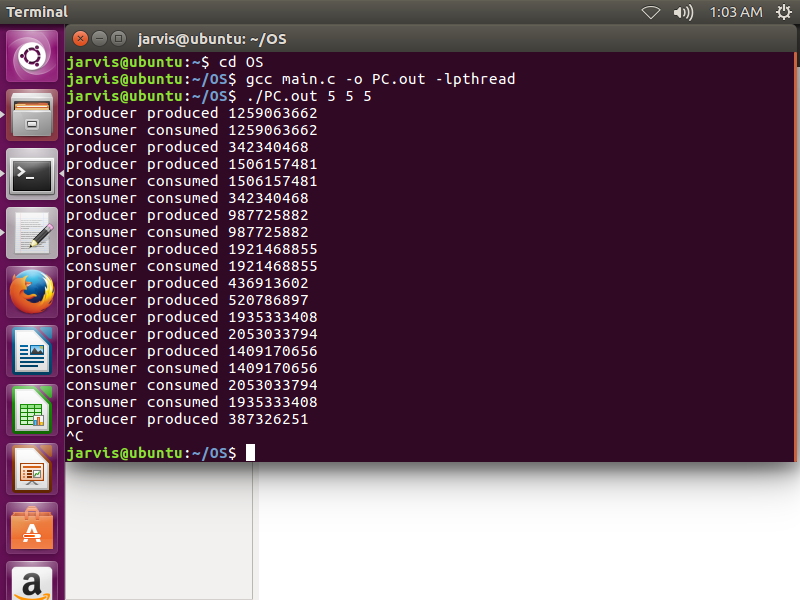
\includegraphics[width=10cm]{pic/555.png}

In this situation, we allocate 5 producers and 5 consumers. The result shows that producer and consumer randomly produce or consume items. But an item must be consumed after being produced(of course!).
\subsection{Producers are more than Consumers}
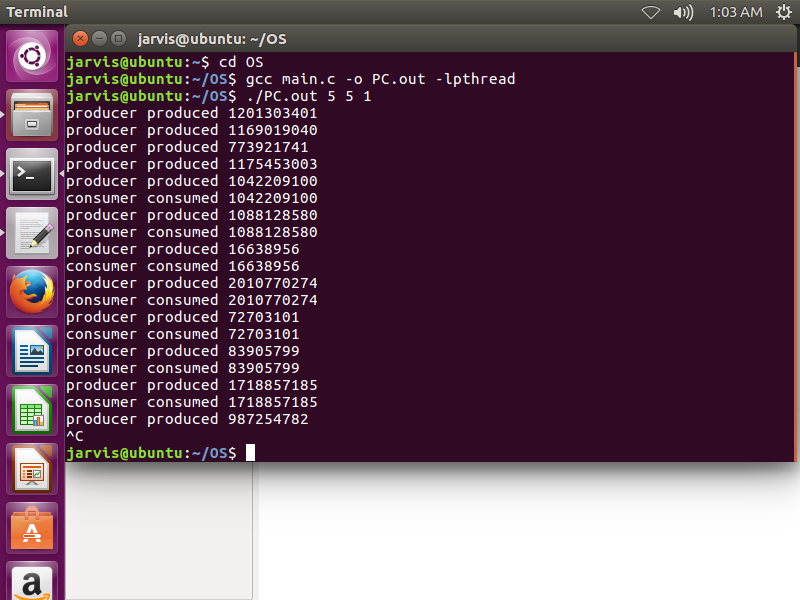
\includegraphics[width=10cm]{pic/551.png}

In this situation, we allocate 5 producers and 1 consumer. The result shows that 5 items are produced first, and the buffer is full. Once an item is consumed, another new item will be produced immediately. So the first 4 items will remains in the bounded buffer.
\subsection{Producers are less that Consumers}
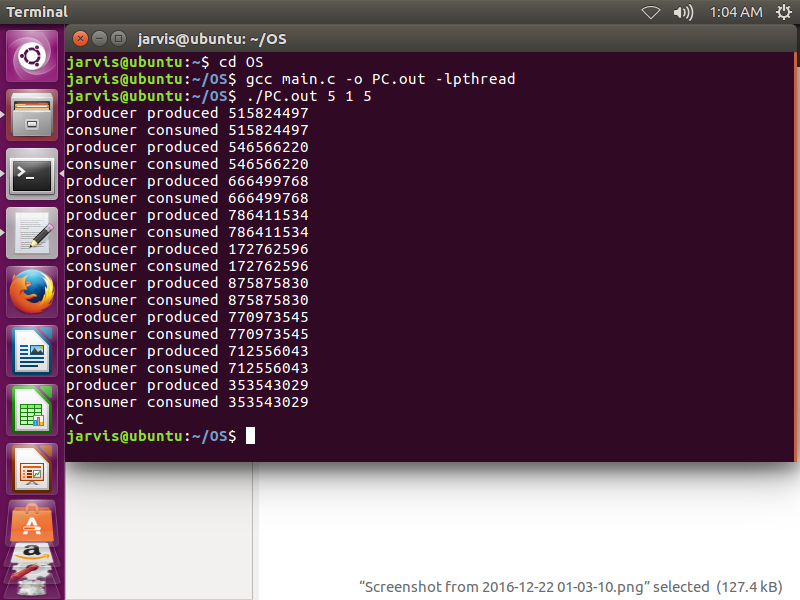
\includegraphics[width=10cm]{pic/515.png}

In this situation, we allocate 1 producers and 5 consumer. An item that is produced will be consumed immediately.
\end{document}
